%% LyX 2.4.4 created this file.  For more info, see https://www.lyx.org/.
%% Do not edit unless you really know what you are doing.
\documentclass[english]{article}
\usepackage[T1]{fontenc}
\usepackage[latin9]{inputenc}
\usepackage{enumitem}
\usepackage{amsmath}
\usepackage{amsthm}
\usepackage{cancel}
\usepackage{geometry}
\geometry{verbose,tmargin=1in,bmargin=1in,lmargin=1in,rmargin=1in}

\makeatletter
%%%%%%%%%%%%%%%%%%%%%%%%%%%%%% Textclass specific LaTeX commands.
\numberwithin{equation}{section}
\numberwithin{figure}{section}
\newlength{\lyxlabelwidth}      % auxiliary length 

%%%%%%%%%%%%%%%%%%%%%%%%%%%%%% User specified LaTeX commands.
\usepackage{fancyhdr}
\usepackage{lastpage}
\pagestyle{fancy}
\usepackage{enumitem}
\usepackage{ifthen}
%sets math fonts to be more readable
\everymath=\expandafter{\the\everymath\displaystyle}
%\DeclareMathSizes{10}{10}{10}{10}
\usepackage{multicol}

\usepackage{tikz}
\usetikzlibrary{plotmarks}
\usepackage{pgfplots}
\pgfplotsset{compat=newest}

\usepackage{calc}
\usepackage[nomessages]{fp}

\usepackage{advdate}    % Advancing/saving dates
\usepackage{datetime}   % Dates formatting
\usepackage{datenumber} % Counters for dates

\usepackage[super]{nth}
% Added by lyx2lyx
\setlength{\parskip}{\smallskipamount}
\setlength{\parindent}{0pt}

\makeatother

\usepackage{babel}
\begin{document}
\renewcommand{\author}{Dr.\,James Ashe}

\newcommand{\classNum}{107}

\newcommand{\classSec}{7 and 10}

\newcommand{\nameType}{Name:}

\newcommand{\examType}{Exam 1}

\renewcommand{\date}{ \formatdate{8}{9}{2014}}

%%First page's header%%%%%%%%%%%%%%%%%%%%%%
\fancypagestyle{firststyle} %%header settings for first pagr
{
	\fancyhead[L]{MTH \classNum{}(\classSec{}) \author{}\\
	\textbf{\examType{}} \date{}}
	\fancyhead[C]{\textbf{\nameType}}
	\setlength{\headsep}{14pt}
}
%%%%%%%%%%%%%%%%%%%%%%%%%%%%%%%%%%%%%%%%%%

%%Next page's header%%%%%%%%%%%%%%%%%%%%%%%
%\setlist{nolistsep}
\lhead{MTH \classNum{}(\classSec{})} 
\chead{\textbf{\nameType}} 
\cfoot{\thepage{}~of~\pageref{LastPage}} 
\setlength{\headsep}{5pt} 
%%%%%%%%%%%%%%%%%%%%%%%%%%%%%%%%%%%%%%%%%%%

%%Various settings; see the preamble for other settings%%%%%
%%\setenumerate[0]{leftmargin=12pt,itemindent=0pt,labelwidth=0pt}
\renewcommand{\labelenumi}{\textbf{\arabic{enumi}.}}
\renewcommand{\labelenumii}{\textbf{\alph{enumii}.}}
\thispagestyle{firststyle}
%%%%%%%%%%%%%%%%%%%%%%%%%%%%%%%%%%%%%%%%%%
\newcommand{\xmax}{10}
\newcommand{\xmin}{-10}
\newcommand{\xstep}{0} %must be xmin+n
\newcommand{\ymax}{10}
\newcommand{\ymin}{-10}
\newcommand{\ystep}{0} %must be ymin+n

\newcommand{\xspace}{\vspace{.5cm}}\newcommand{\vennScale}{0.65}\emph{You must show your work to receive
credit. Unless stated otherwise, each problem is worth 4 points. }
\begin{enumerate}[resume]
\item {[}3 points each{]} Use the provided diagrams to shade in the region
corresponding to the indicated set.\begin{multicols}{2} \newcommand{\fudgeSpace}{-.5cm}

\begin{enumerate}
\item \textbf{$A\cup B$}

\hspace{\fudgeSpace}%%%%A uncolored; B uncolored%%%%%
\begin{tikzpicture}[scale=\vennScale]
	\def\circleA{(0,0) circle (1.5)} %A
	\def\circleB{(0:2) circle (1.5)} %B

	\colorlet{circle edgeA}{black!75} 
	\colorlet{circle areaA}{red!100}
	\colorlet{circle edgeB}{black!75} 
	\colorlet{circle areaB}{green!100}

	\tikzset{
		filledA/.style={fill=circle areaA, draw=circle edgeA, thick},
		filledB/.style={fill=circle areaB, draw=circle edgeB, thick},
		outlineA/.style={draw=circle edgeA, thick},
		outlineB/.style={draw=circle edgeB, thick},
	}

	\begin{scope}[fill opacity=0.5]         
			%\fill[filledB] \circleB;    
			%\fill[filledA] \circleA;
	\end{scope}

	\draw[outlineA] \circleA node {$A$}; 
	\draw[outlineB] \circleB node {$B$}; 
	%\node[anchor=south] at (current bounding box.north) {$A \cap B$}; 
	\draw[thick] (-2,-2) rectangle (4,2) node[anchor=south east] at (current bounding box.south east) {$U$}; 
\end{tikzpicture} 
\item $A\cap B$

\hspace{\fudgeSpace}%%%%A uncolored; B uncolored%%%%%
\begin{tikzpicture}[scale=\vennScale]
	\def\circleA{(0,0) circle (1.5)} %A
	\def\circleB{(0:2) circle (1.5)} %B

	\colorlet{circle edgeA}{black!75} 
	\colorlet{circle areaA}{red!100}
	\colorlet{circle edgeB}{black!75} 
	\colorlet{circle areaB}{green!100}

	\tikzset{
		filledA/.style={fill=circle areaA, draw=circle edgeA, thick},
		filledB/.style={fill=circle areaB, draw=circle edgeB, thick},
		outlineA/.style={draw=circle edgeA, thick},
		outlineB/.style={draw=circle edgeB, thick},
	}

	\begin{scope}[fill opacity=0.5]         
			%\fill[filledB] \circleB;    
			%\fill[filledA] \circleA;
	\end{scope}

	\draw[outlineA] \circleA node {$A$}; 
	\draw[outlineB] \circleB node {$B$}; 
	%\node[anchor=south] at (current bounding box.north) {$A \cap B$}; 
	\draw[thick] (-2,-2) rectangle (4,2) node[anchor=south east] at (current bounding box.south east) {$U$}; 
\end{tikzpicture} 
\item $A'$

\hspace{\fudgeSpace}%%%%A uncolored; B uncolored%%%%%
\begin{tikzpicture}[scale=\vennScale]
	\def\circleA{(0,0) circle (1.5)} %A
	\def\circleB{(0:2) circle (1.5)} %B

	\colorlet{circle edgeA}{black!75} 
	\colorlet{circle areaA}{red!100}
	\colorlet{circle edgeB}{black!75} 
	\colorlet{circle areaB}{green!100}

	\tikzset{
		filledA/.style={fill=circle areaA, draw=circle edgeA, thick},
		filledB/.style={fill=circle areaB, draw=circle edgeB, thick},
		outlineA/.style={draw=circle edgeA, thick},
		outlineB/.style={draw=circle edgeB, thick},
	}

	\begin{scope}[fill opacity=0.5]         
			%\fill[filledB] \circleB;    
			%\fill[filledA] \circleA;
	\end{scope}

	\draw[outlineA] \circleA node {$A$}; 
	\draw[outlineB] \circleB node {$B$}; 
	%\node[anchor=south] at (current bounding box.north) {$A \cap B$}; 
	\draw[thick] (-2,-2) rectangle (4,2) node[anchor=south east] at (current bounding box.south east) {$U$}; 
\end{tikzpicture} 
\item \textbf{$(A\cup B)'$}

\hspace{\fudgeSpace}%%%%A uncolored; B uncolored%%%%%
\begin{tikzpicture}[scale=\vennScale]
	\def\circleA{(0,0) circle (1.5)} %A
	\def\circleB{(0:2) circle (1.5)} %B

	\colorlet{circle edgeA}{black!75} 
	\colorlet{circle areaA}{red!100}
	\colorlet{circle edgeB}{black!75} 
	\colorlet{circle areaB}{green!100}

	\tikzset{
		filledA/.style={fill=circle areaA, draw=circle edgeA, thick},
		filledB/.style={fill=circle areaB, draw=circle edgeB, thick},
		outlineA/.style={draw=circle edgeA, thick},
		outlineB/.style={draw=circle edgeB, thick},
	}

	\begin{scope}[fill opacity=0.5]         
			%\fill[filledB] \circleB;    
			%\fill[filledA] \circleA;
	\end{scope}

	\draw[outlineA] \circleA node {$A$}; 
	\draw[outlineB] \circleB node {$B$}; 
	%\node[anchor=south] at (current bounding box.north) {$A \cap B$}; 
	\draw[thick] (-2,-2) rectangle (4,2) node[anchor=south east] at (current bounding box.south east) {$U$}; 
\end{tikzpicture} 
\end{enumerate}
\end{multicols}
\item {[}3 points each{]} Let $U=\{a,b,c,x,y,z\}$ be the universal set,
and $A=\{a,b,c\}$, $B=\{c,x,y\}$, $C=\{y,z\}$ be subsets of $U$.
Find the indicated set.

\begin{enumerate}
\item $A\cup B$\xspace\xspace
\item $A\cap B$\xspace\xspace
\item $A\cap C$\xspace\xspace
\item $A'$\xspace\xspace
\item $(A\cup B)'$\xspace\xspace
\end{enumerate}
\item A survey of $1000$ students finds that $700$ like pizza, $600$
like hamburgers, and $400$ like both.\begin{multicols}{1}

\begin{enumerate}
\item []Use the provided Venn diagram to label and write the appropriate
numbers in the four regions

\begin{enumerate}
\item []%%%%A uncolored; B uncolored%%%%%
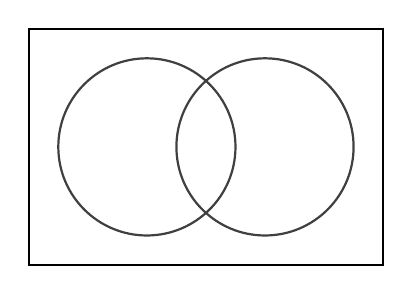
\begin{tikzpicture}[scale=.75]
	\def\circleA{(0,0) circle (1.5)} %A
	\def\circleB{(0:2) circle (1.5)} %B

	\colorlet{circle edgeA}{black!75} 
	\colorlet{circle areaA}{red!100}
	\colorlet{circle edgeB}{black!75} 
	\colorlet{circle areaB}{green!100}

	\tikzset{
		filledA/.style={fill=circle areaA, draw=circle edgeA, thick},
		filledB/.style={fill=circle areaB, draw=circle edgeB, thick},
		outlineA/.style={draw=circle edgeA, thick},
		outlineB/.style={draw=circle edgeB, thick},
	}

	\begin{scope}[fill opacity=0.5]         
			%\fill[filledB] \circleB;    
			%\fill[filledA] \circleA;
	\end{scope}

	\draw[outlineA] \circleA node {$$}; 
	\draw[outlineB] \circleB node {$$}; 
	%\node[anchor=south] at (current bounding box.north) {$A \cap B$}; 
	\draw[thick] (-2,-2) rectangle (4,2) node[anchor=south east] at (current bounding box.south east) {$$}; 
\end{tikzpicture} \columnbreak
\end{enumerate}
\item How many students like pizza or hamburgers? \vfill
\item How many students like pizza but not hamburgers?\vfill
\item How many students like neither pizza nor hamburgers?\xspace\vfill
\end{enumerate}
\end{multicols}
\end{enumerate}
\vfill\newpage
\begin{enumerate}[resume]
\item Out of $500$ MHU students, $200$ are taking a history class, $200$
are taking a math class, and $150$ are taking a biology class. $50$
students are taking all three. $80$ students are taking both history
and math. $40$ students are taking biology but neither math nor history.
$90$ students are taking both history and biology.\begin{multicols}{2}

\begin{enumerate}
\item []Use the provided Venn diagram to write the appropriate numbers
in the eight regions.\xspace

\begin{enumerate}
\item []\def\firstcircle{(90:1.75cm) circle (2.5cm)} 
\def\secondcircle{(210:1.75cm) circle (2.5cm)} 
\def\thirdcircle{(330:1.75cm) circle (2.5cm)}

\begin{tikzpicture}[scale=.65]    
\begin{scope}     
	\fill[white]\firstcircle;       
	\fill[white] \secondcircle;       
	\fill[white] \thirdcircle;     
\end{scope}     
\begin{scope}
	\clip 
	\secondcircle;       
	\fill[white] 
	\firstcircle;     
\end{scope}     
\begin{scope}       
	\clip 
	\secondcircle;       
	\fill[white] 
	\thirdcircle;     
\end{scope}     
\begin{scope}       
	\clip 
	\firstcircle;       
	\fill[white] 
	\thirdcircle;     
\end{scope}     
\begin{scope}       
	\clip \firstcircle;       
	\clip \secondcircle;       
	\fill[white] \thirdcircle;     
\end{scope}     
\draw 
	\firstcircle node[text=black] {$H$} node[above=10pt] {$$};     
\draw 
	\secondcircle node [text=black,below left] {$M$} node[below left=10pt] {$$};     
\draw 
	\thirdcircle node [text=black,below right] {$B$} node[below right=10pt] {$$};     
%%\begin{scope}[font=\small]       
	%\node(0,0) {$50$}; %AnBnC       
	%\draw(30:1.5cm) node {$140$}; %AnC       
	%\draw(150:1.5cm) node {$130$}; %AnB       
	%\draw(270:1.5cm) node {$80$}; %BnC    
%%\end{scope}

\draw[thick] (-4.8,-3.55) rectangle (4.75,4.4) node[anchor=south east] at (current bounding box.south east) {$U$} node[anchor=north west] at (current bounding box.north west) {$$}; 

\end{tikzpicture}\columnbreak
\end{enumerate}
\item How many students are taking only history?\vfill
\item How many students are taking history or Math?\vfill
\item How many students are not taking history, math, or biology?\xspace\vfill
\end{enumerate}
\end{multicols}
\end{enumerate}
\vfill
\begin{enumerate}[resume]
\item Find the value of each of the following:\begin{multicols}{2}

\begin{enumerate}
\item $\frac{4!}{0!}$\xspace\xspace
\item $\frac{27!}{4!25!}$\xspace\xspace
\item $\frac{195!}{193!}$\xspace\xspace
\item $_{6}C_{1}$\xspace\xspace
\end{enumerate}
\end{multicols}
\end{enumerate}
\xspace\xspace
\begin{enumerate}[resume]
\item A six-sided dice is thrown, a quarter is flipped, and a card is drawn
from a standard $52$ card deck. How many different outcomes are possible?\xspace\xspace
\end{enumerate}
\vfill
\begin{enumerate}[resume]
\item There are $10$ pigs competing at the county fair in the ``that's
some pig'' contest. 

\begin{enumerate}
\item If the judges see each pig once and only once, how many different
ways can they see all the pigs?\xspace\xspace\xspace
\item The judges will award \nth{1}, \nth{2}, and \nth{3} place prizes.
How many different ways can the prizes be awarded.\xspace\xspace\xspace
\end{enumerate}
\end{enumerate}
\vfill\newpage
\begin{enumerate}[resume]
\item A bowling league has seven teams. If every team must play every other
team once in the first round of league play, how many games must be
scheduled?
\end{enumerate}
\vfill
\begin{enumerate}[resume]
\item A $5$ player team must be chosen from a group of $8$ offensive players
and $7$ defensive players. How many teams are possible if the team
must consist of the following?

\begin{enumerate}
\item $5$ offensive players.\xspace\xspace
\item $3$ offensive players and $2$ defensive players.\xspace\xspace
\item Any mix of offensive and defensive players.\xspace\xspace
\end{enumerate}
\end{enumerate}
\vfill
\begin{enumerate}[resume]
\item Each student at State University has a student ID number consisting
of \emph{four} digits (the digits can be repeated) followed by two
of the letters $A$, $B$, and $C$ (letters cannot be repeated).
How many different student numbers are possible?\vfill
\end{enumerate}

\section*{Honor Statement}

\emph{On my honor, I have neither given nor received any academic
aid or information that would violate the Honor Code of Mars Hill
University.}
\begin{itemize}
\item []Signature:\underline{\hspace{7cm}}\vfill
\end{itemize}

\end{document}
